\section{Introduction to \mbox{Mote Runner}}
\begin{frame}[fragile]
  \frametitle{Mote Runner}
  \begin{itemize}
    \item An OS and a runtime and development environment for WSN
    \item Key features:
    \begin{itemize}
      \item Support for RT constraints \& energy awareness
      \item Portability thanks to a VM that abstracts the HW
      \item Event oriented programming paradigm
      \item High level coding (Java - C\#)
      \item Debugging \& simulation environments
    \end{itemize}
    \item It’s still in beta and is evolving towards IoT
  \end{itemize}
\end{frame}

\begin{frame}[fragile]
  \frametitle{Mote Runner Operating System}
  \begin{columns}
    \begin{column}{.48\linewidth}
    	\begin{itemize}
	    	\item Mote Runner system provides:
	    	\begin{itemize}
		    	\item A Virtual Machine for executing byte codes
		    	\item An Operating System for:
		    	\begin{itemize}
			    	\item  organizing access to different devices 
			    	\item scheduling the various activities
		    	\end{itemize} 
		    \end{itemize}
    	\end{itemize}
    \end{column}
    \hfill
    \begin{column}{.5\linewidth}
    	\begin{figure}
	  \centering
	  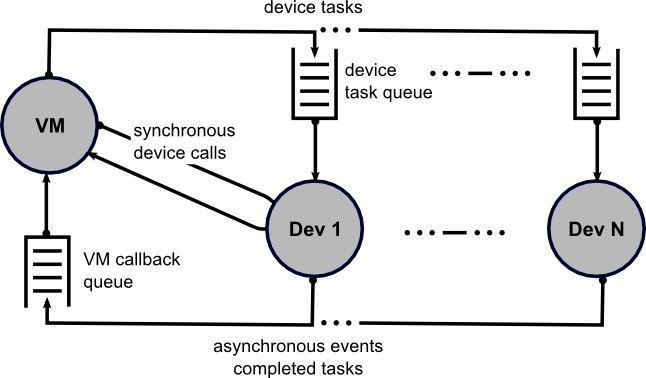
\includegraphics[width=\textwidth]{img/vm-dev.jpg}
    	\end{figure}
    \end{column}
  \end{columns}
\end{frame}

\begin{frame}[fragile]
  	\frametitle{Device Model}
  	\begin{itemize}
  		\item The OS assumes that all devices have the following states
  	\end{itemize}
  	\begin{figure}
  		\centering
   		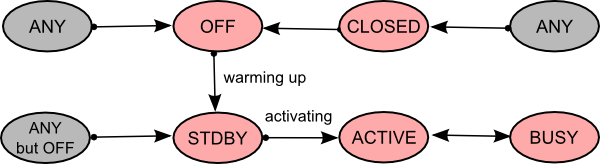
\includegraphics[width=0.6\textwidth]{img/sdev-states.png}
  	\end{figure}
  	\begin{itemize}
 		\item The OS manage implicitely most of the state changes:
	 	 \begin{itemize}
	  		\item Makes sure that the device ramp up happens before the requested time
			\item Keeps device in states with the lowest energy consumption
			\item Application, however, can put devices into the states CLOSED, OFF and STDBY
		\end{itemize}
	\end{itemize}
\end{frame}

\begin{frame}[fragile]
  \frametitle{Mote Runner}
  \begin{columns}
    \begin{column}{.5\linewidth}
    	\begin{figure}
	  \centering
	  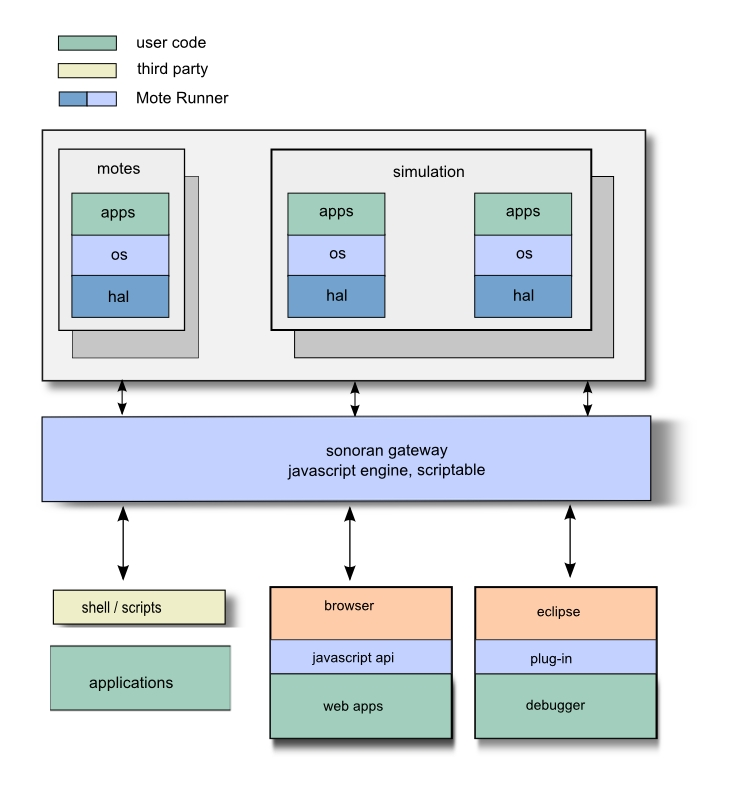
\includegraphics[width=\textwidth]{img/overview.jpg}
    	\end{figure}
    \end{column}
    \hfill
    \begin{column}{.5\linewidth}
    	\begin{figure}
	  \centering
	  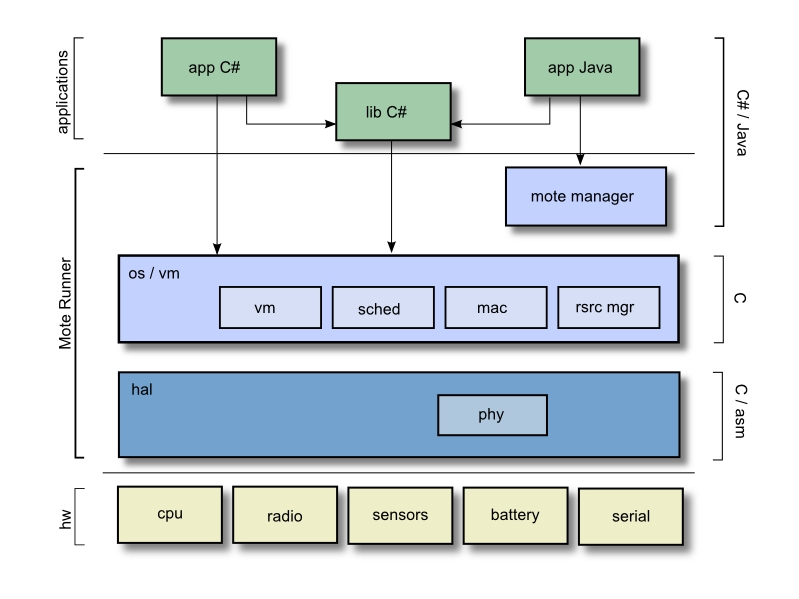
\includegraphics[width=\textwidth]{img/onmote.jpg}
    	\end{figure}
    \end{column}
  \end{columns}
\end{frame}

\begin{frame}[fragile]
  \frametitle{Mote Runner - v.11, v.13 beta}
  \begin{itemize}
    \item They support IEEE 802.15.4
    \begin{itemize}
    	\item exposing a low radio level API that can be used to implement custom MAC layer
    	\item dropping messages with header structure not 802.15.4 compliant in the radio stack 
    \end{itemize}
    \item Offer Hopi
    \begin{itemize}
    	\item A multi-hop data gathering protocol
    	\item Used to collect data from motes setting automatically a tree network
    \end{itemize}
  \end{itemize}
\end{frame}

\begin{frame}[fragile]
  \frametitle{Mote Runner - v.17.1.8c (latest)}
  \begin{itemize}
    \item Supports only two platforms: IMST \& Blipper
    \item It’s based on a different radio layer: LoRa\texttrademark
    \item It offers a build-in MAC layer: LRSC - Low Range Signaling \& Control
    \begin{itemize}
    	\item It supports only a network topology: the LRSC one
    	\item The offered API is poor since the radio is hidden in the firmware (not compatible with previous versions)
    \end{itemize}

  \end{itemize}
\end{frame}

\begin{frame}[fragile]
  \frametitle{LRSC - Architecture}
  \begin{columns}
    \begin{column}{.48\linewidth}
    	\begin{itemize}
	  \item Gateways (GW) are connected to server on IP
	  \item Motes comunicate with server in tunneling TCP/UDP over IP
	  \item Motes comunicate with GW with LoRa single-hop
    	\end{itemize}
    \end{column}
    \hfill
    \begin{column}{.48\linewidth}
    	\begin{figure}
	  \centering
	  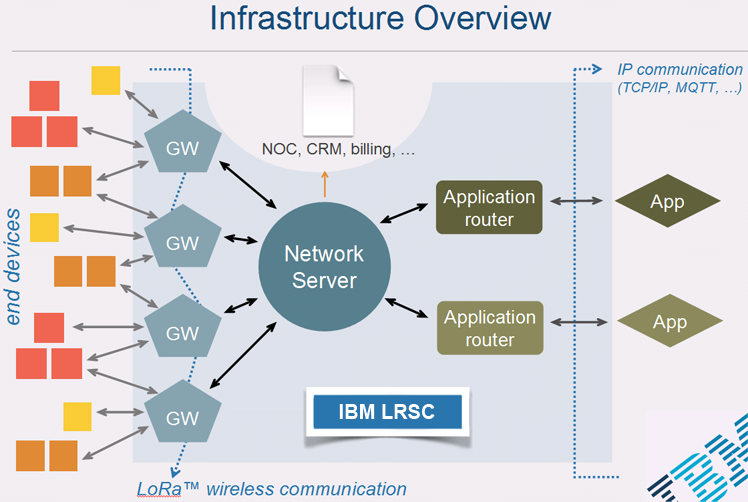
\includegraphics[width=\linewidth]{img/LRSC_infrastructure.png}
    	\end{figure}

    \end{column}
  \end{columns}
\end{frame}

\begin{frame}[fragile]
  \frametitle{IBM LRSC}
    	\begin{itemize}
	  \item The Long Range Signaling and Control (LRSC) system is a network infrastructure which relies on LoRa\texttrademark, modulation technology developed by Semtech for wireless bidirectional communication over distances of up to 15 km in semi-rural environments and up to five km in dense urban environments.
	  \item All communication is generally bi-directional, although uplink communication from end devices to the network server is strongly favored, and is based on LoRa.
    	\end{itemize}
   
\end{frame}


\begin{frame}[fragile]
  \frametitle{LRSC network simulation}
    	The Mote Runner SDK ships with:
    	\begin{itemize}
	  \item LoRa Mac library providing an API for accessing a LRSC network. 
	  \item LIP shell interface to control the Mac from the Mote Runner shell MRSH.
    	\end{itemize}
  The main constraint for our intial purpose depends on the fact that the end devices cannot communicate directly. Any message should be sent over the LRSC network.
\end{frame}

\begin{frame}[fragile]
  \frametitle{LoRa\texttrademark}
  \begin{columns}
    \begin{column}{.48\linewidth}
      \begin{itemize}
	\item LoRa\texttrademark Alliance
	\begin{itemize}
	  \item Target: IoT,  machine-to-machine (M2M), smart city, and industrial applications
	  \item Intiated to standardize Low Power Wide Area Networks (LPWAN)
	\end{itemize}
      \end{itemize}
    \end{column}
    \hfill
    \begin{column}{.48\linewidth}
    	\begin{figure}
	  \centering
	  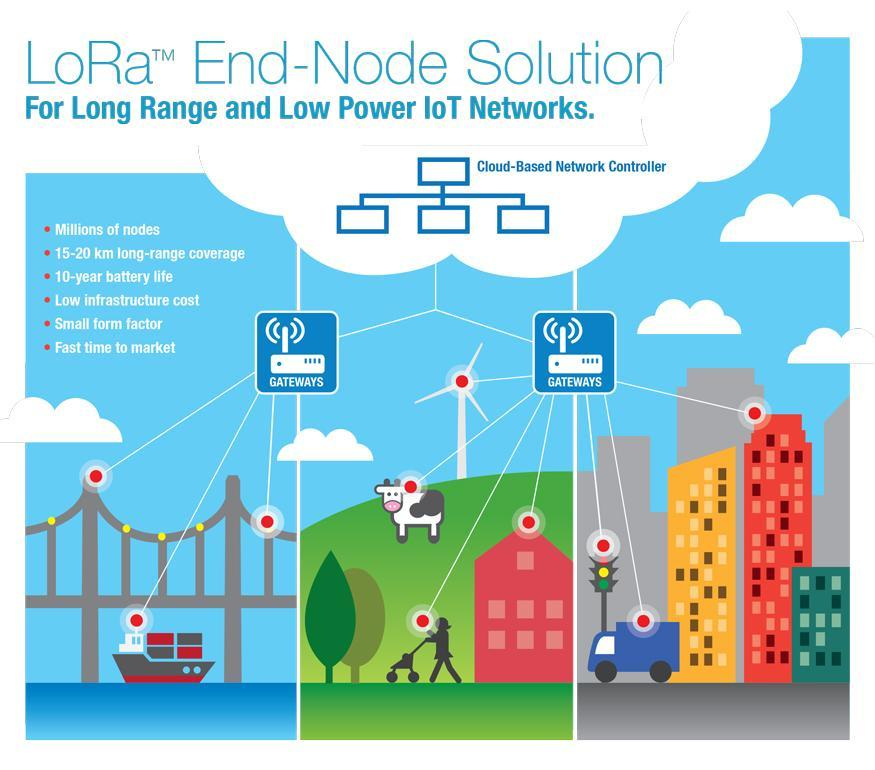
\includegraphics[width=\linewidth]{img/lora.jpg}
    	\end{figure}

    \end{column}
  \end{columns}
\end{frame}

\begin{frame}[fragile]
  \frametitle{LoRa\texttrademark}
  \begin{itemize}
    \item LoRa\texttrademark Technology
    \begin{itemize}
      \item LoRaWAN pledeges to extend the radio range by 10x while using only one third of the power used by competing solutions 
      \item Star (of stars) topology
      \item Gateways relay messages between end-devices and a central network server
      \item Communication between end-devices and gateways is spread out on different frequency channels and data rates.
      \item Data rates: 0.3 - 50 kbps
    \end{itemize}
  \end{itemize}
\end{frame}

\begin{frame}[fragile]
  \frametitle{LoRa\texttrademark}
  \begin{itemize}
    \item ...and more
    \begin{itemize}
      \item adaptive data rate (ADR)
      \item secure communication (on network and application layers and end-point device key)
      \item three classes of end-point devices.
      \item More info on http://lora-alliance.org/
    \end{itemize}
  \end{itemize}
\end{frame}

\begin{frame}[fragile]
  \frametitle{Mote Runner - Conclusion}
  \vspace{-1em}
  \begin{itemize}
    \item For the purpose of this work (TAKS \& WIDS):
    \begin{itemize}
    	\item MR allows dynamic reprogramming of motes with a control server using WLIP
    	\item v.17.1.8c is not suitable
    	\begin{itemize}
	  \item LoRa is available only for a limited number of platforms (until now!)
	  \item LRSC doesn’t permit to customize the MAC behaviour
	  \item The radio is not exposed
    	\end{itemize}
    	\item v.11, v.13 are better choices:
    	\begin{itemize}
	  \item radio interface could be used to implement an 802.15.4 MAC with TAKS support
	  \item this MAC could be used to build upper layer with WIDS
    	\end{itemize}
    \end{itemize}
    \item This does not exclude a future integration with LoRa-LRSC
  \end{itemize}
\end{frame}

\begin{frame}[fragile]
  \frametitle{Mote Runner}
  \begin{itemize}
    \item 
  \end{itemize}
\end{frame}